\chapter{Étude conceptuelle}
\label{sec:troisiemechapitre}

\section{Introduction}



\section{Conception de la plateforme : vue statique}

\vspace{5mm}

\subsection{Diagramme de déploiment}

\vspace{5mm}

\subsection{Diagramme de classes}
\vspace{5mm}






\section{Conception de la plateforme : vue dynamique}
La vue dynamique met l’accent sur le comportement dynamique du système en illustrant les collaborations entre les objets et les changements apportés à états internes d'objets. Durant cette phase, nous décrirons le comportement général du système en présentant les diagramme de séquences.
\vspace{5mm}

\subsection{Diagramme de séquences}
\vspace{5mm}


\subsubsection{Diagramme de séquence << Ajouter une tâche >>:}
\vspace{5mm}
\begin{itemize}[label=$\bullet$]
    \item \textbf{Diagramme de séquence système: }
    \par \vspace{2mm}
    La figure \ref{fig:tasksys} illustre le diagramme de séquence système d'ajouter une tâche.
    \begin{figure}[H]
  \centering
  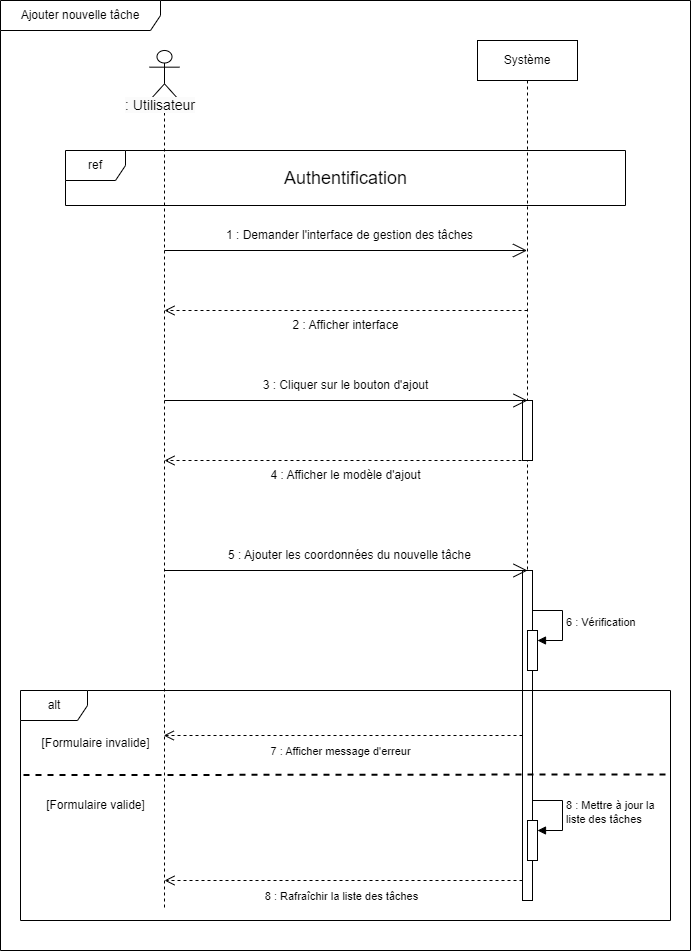
\includegraphics[scale=0.6]{chapitre3/figuresChap3/nouvelle tache (sys).png}
  \caption{Diagramme de séquence système de << Ajouter une tâche >>}   
  \label{fig:tasksys}
\end{figure}
    
    \item \textbf{Diagramme de séquence détaillé: }
    \par \vspace{2mm}
    La figure \ref{fig:taskdetail} illustre le diagramme de séquence détaillé d'ajouter une tâche.
    \begin{figure}[H]
  \centering
  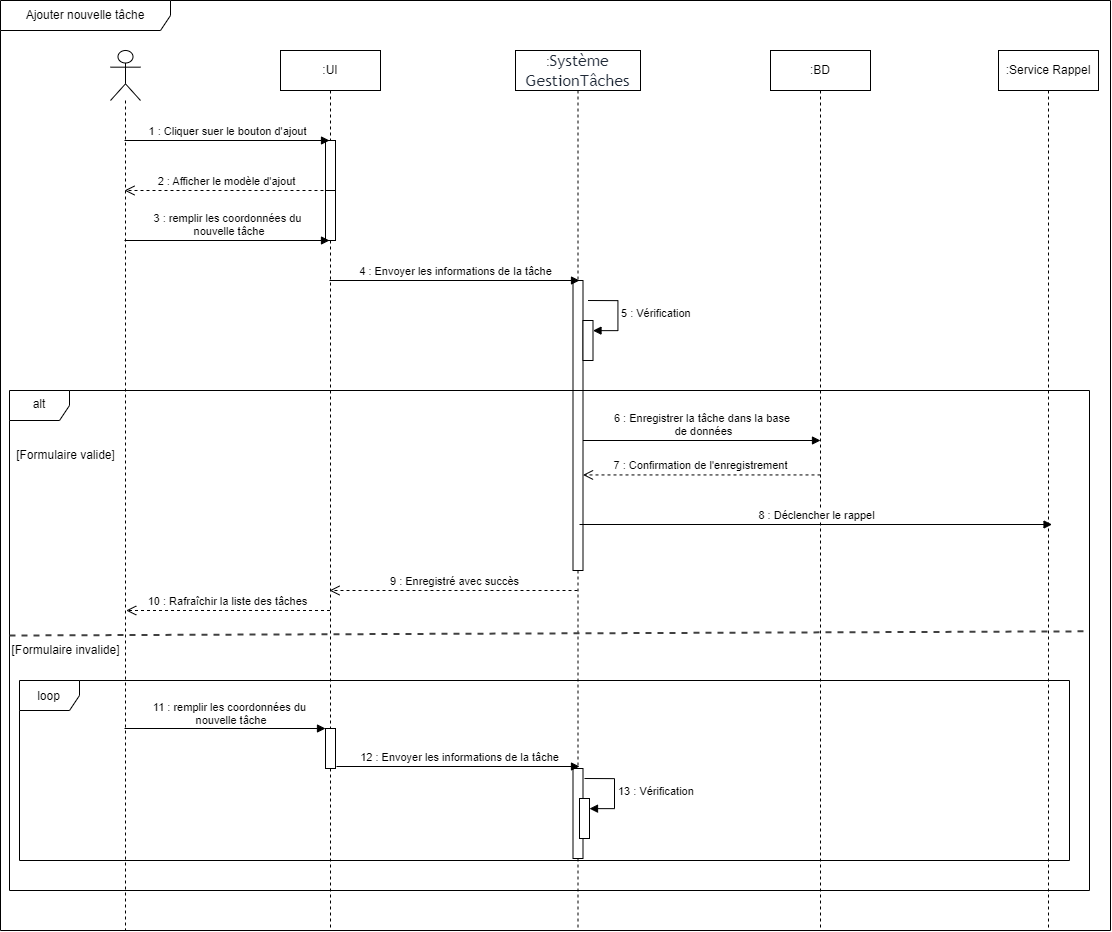
\includegraphics[scale=0.45]{chapitre3/figuresChap3/addtaskFINAL.png}
  \caption{Diagramme de séquence détaillé de << Ajouter une tâche >>}   
  \label{fig:taskdetail}
\end{figure}
\end{itemize}


\vspace{5mm}
\subsubsection{Diagramme de séquence << Ajouter une note >>:}
\vspace{5mm}
\begin{itemize}[label=$\bullet$]
    \item \textbf{Diagramme de séquence système: }
    \par \vspace{2mm}
    La figure \ref{fig:notesys} illustre le diagramme de séquence système d'ajouter une note.
    \begin{figure}[H]
  \centering
  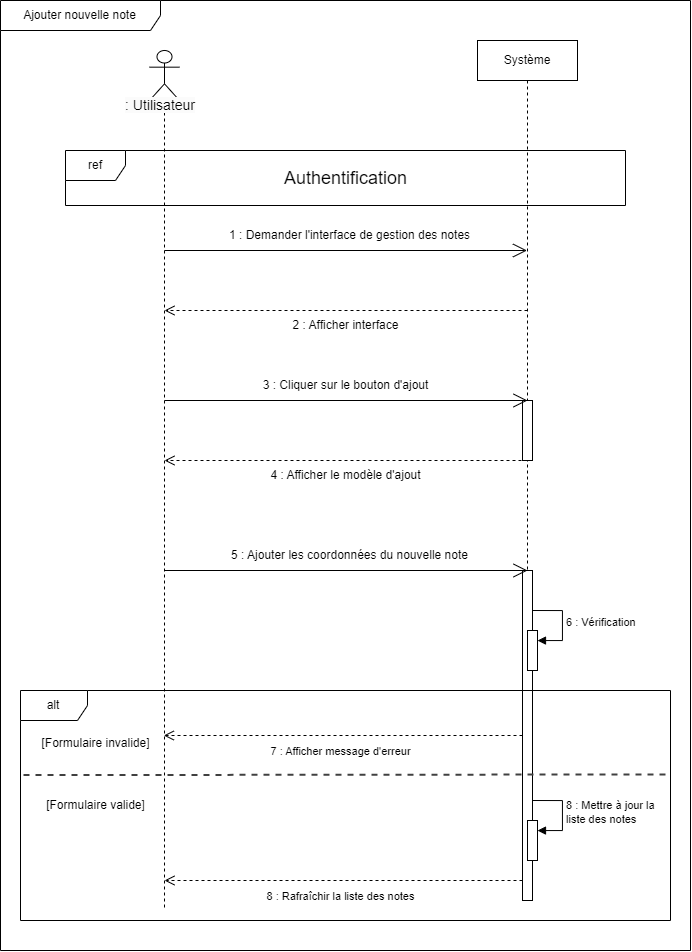
\includegraphics[scale=0.6]{chapitre3/figuresChap3/addnotesys.png}
  \caption{Diagramme de séquence système de << Ajouter une note >>}   
  \label{fig:notesys}
\end{figure}

\item \textbf{Diagramme de séquence détaillé: }
    \par \vspace{2mm}
    La figure \ref{fig:notedetail} illustre le diagramme de séquence détaillé d'ajouter une note.
\begin{figure}[H]
  \centering
  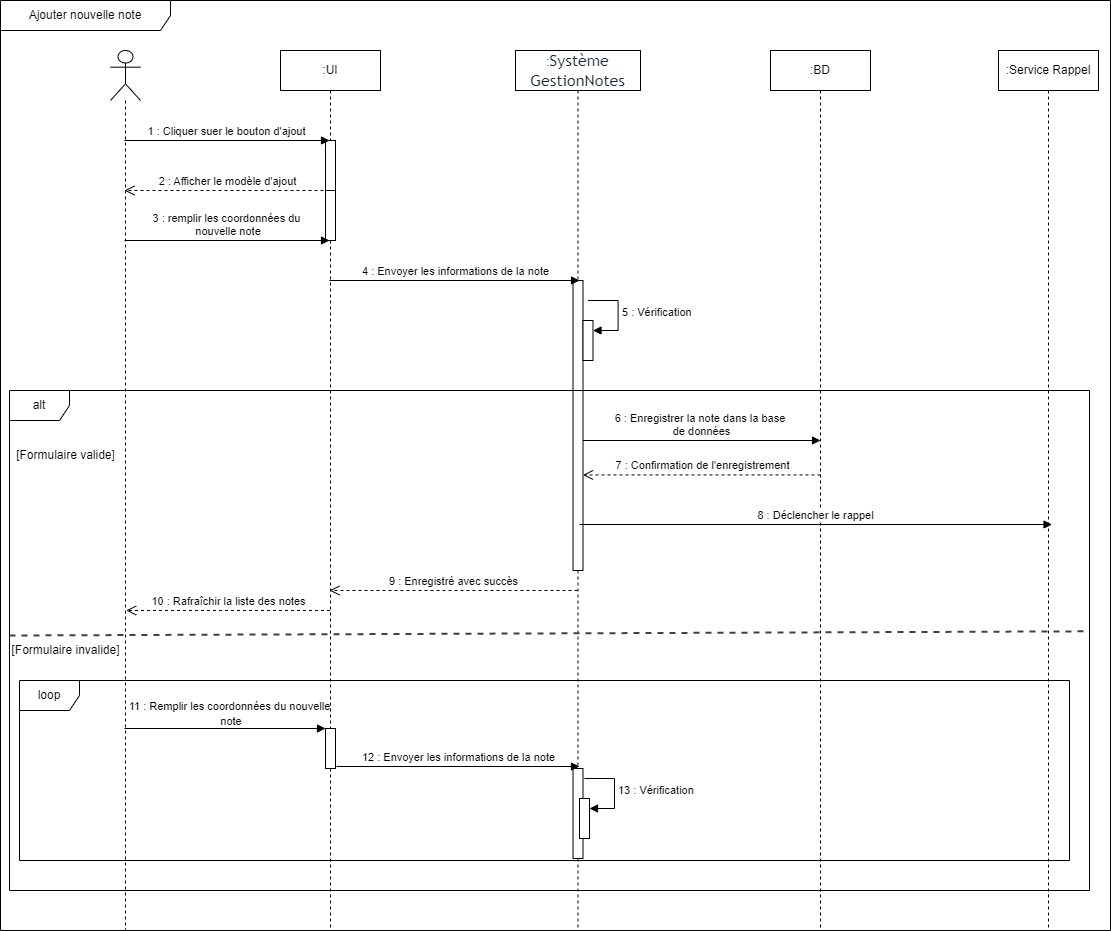
\includegraphics[scale=0.45]{chapitre3/figuresChap3/addnotefinal.png}
  \caption{Diagramme de séquence détaillé de << Ajouter une note >>}   
  \label{fig:notedetail}
\end{figure}












\end{itemize}

















\vspace{5mm}
\subsubsection{Diagramme de séquence << Classification des documents >>:}
\vspace{5mm}
\begin{itemize}[label=$\bullet$]
 \item \textbf{Diagramme de séquence détaillé: }
    \par \vspace{2mm}
    La figure \ref{fig:classdetail} illustre le diagramme de séquence détaillé d'ajouter une tâche.
    \begin{figure}[H]
  \centering
  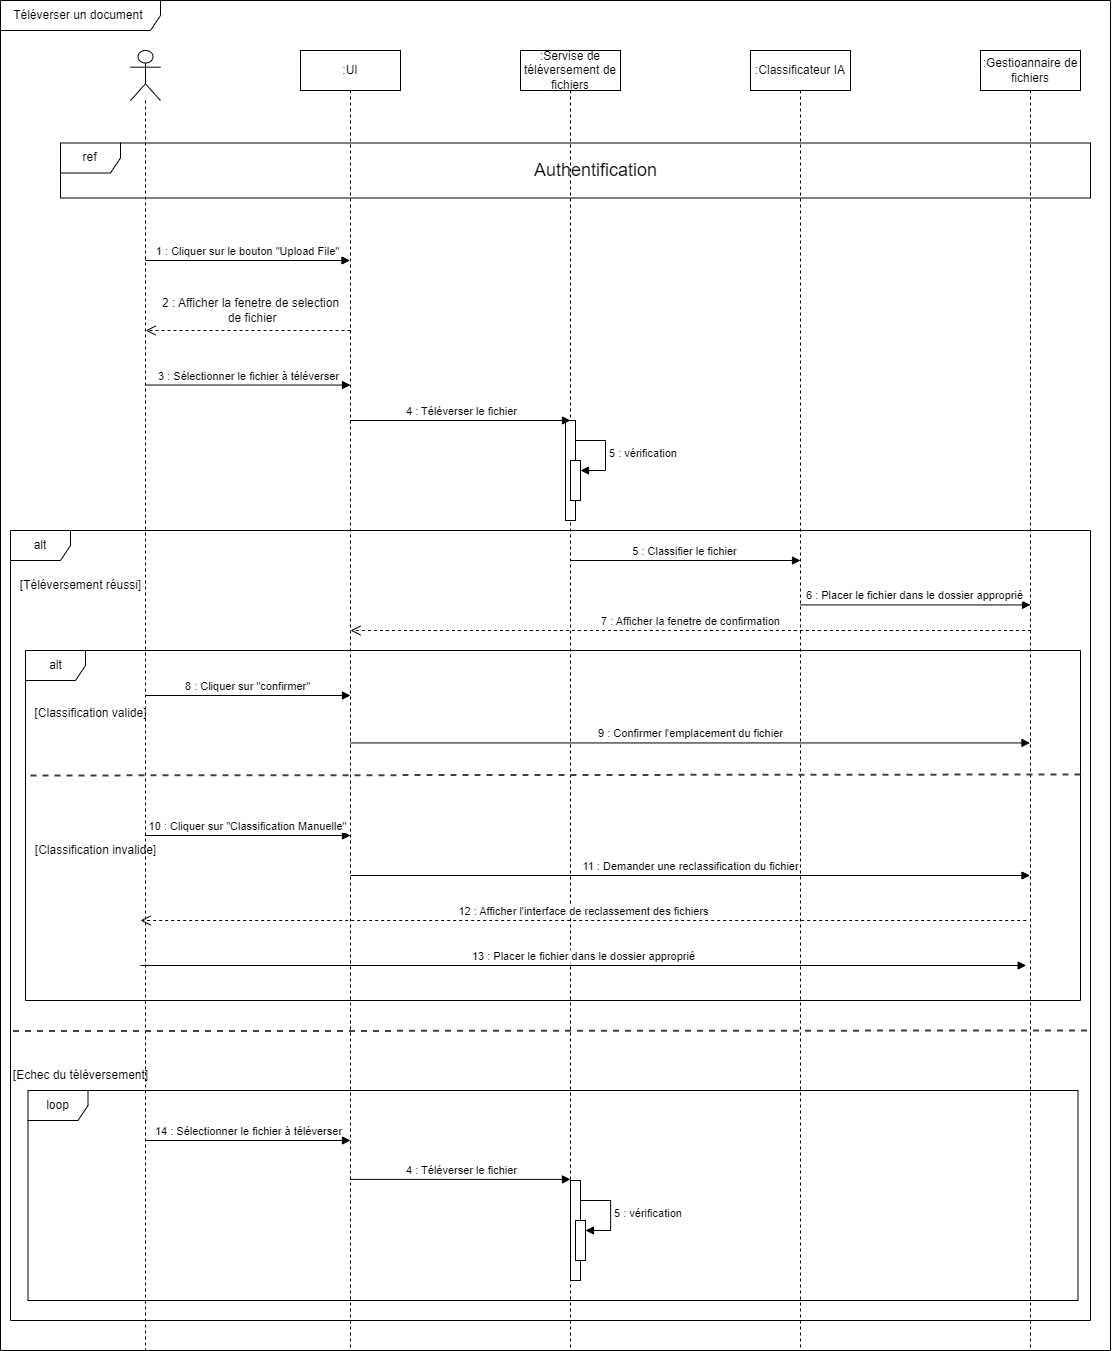
\includegraphics[scale=0.45]{chapitre3/figuresChap3/docmanagerfinal.png}
  \caption{Diagramme de séquence détaillé de << Classification des documents >>}   
  \label{fig:classdetail}
\end{figure}
\end{itemize}

\newpage


\section{Diagramme d'état/transition}
Les diagrammes d’états-transitions d’UML décrivent le comportement interne d’un objet à l’aide d’un automate à états finis. Ils présentent les séquences possibles d’états et d’actions. \\ Le passage d’un état vers l’autre est matérialisé par une transition. \\ Les transitions sont déclenchées par la fin d’une transition et entraînent le début immédiat d’une autre (automatique).
\vspace{8mm}

\subsubsection{Diagramme d'état/transition : objet tâche}
\vspace{5mm}
La figure \ref{fig:etat tache} illustre l'état transition de l'objet << tâche >>:


\begin{figure}[H]
  \centering
  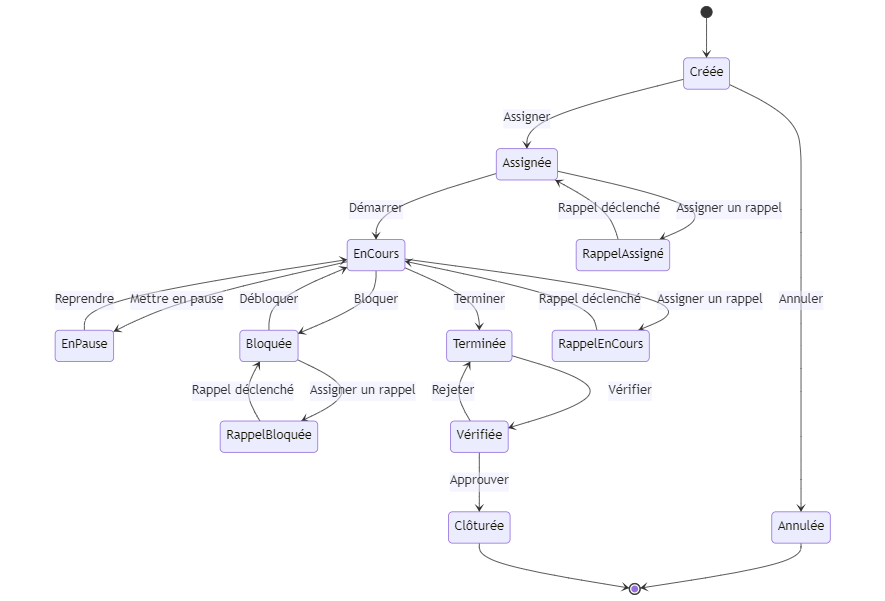
\includegraphics[scale=0.6]{chapitre2/figuresChap2/mermaid-diagram-2024-05-20-131857.png}
  \caption{Etat transition de l'objet << tâche >>}   
  \label{fig:etat tache}
\end{figure}


\section{Conclusion}
Au cours de ce chapitre, nous avons détaillé le modèle conceptuel de notre projet qui va être utilisé dans le développement de la plateforme.
Dans le prochain chapitre, nous allons étudier la partie réalisation qui sera traduite par la présentation de l'environnement du travail et les interfaces réalisées.
 




